\documentclass[10pt,journal,compsoc]{IEEEtran}

\ifCLASSOPTIONcompsoc
  \usepackage[nocompress]{cite}
  \usepackage{tabularx}
  \usepackage{array}
  \usepackage{hyperref}
  \usepackage{graphicx}
  \usepackage{caption}
 \usepackage[numbers]{natbib}
\bibliographystyle{plainnat}
\else
  % normal IEEE
  \usepackage{cite}
\fi


% *** GRAPHICS RELATED PACKAGES ***
%
\ifCLASSINFOpdf
\else

\fi
\newcommand\MYhyperrefoptions{bookmarks=true,bookmarksnumbered=true,
pdfpagemode={UseOutlines},plainpages=false,pdfpagelabels=true,
colorlinks=true,linkcolor={black},citecolor={black},urlcolor={black},
pdftitle={Bare Demo of IEEEtran.cls for Computer Society Journals},%<!CHANGE!
pdfsubject={Typesetting},%<!CHANGE!
pdfauthor={Michael D. Shell},%<!CHANGE!
pdfkeywords={Computer Society, IEEEtran, journal, LaTeX, paper,
             template}}%<^!CHANGE!

\hyphenation{optical networks semiconductor}


\begin{document}
\title{Visualización de datos: Caso Cáncer Pulmonar}


\author{Jose~Perez Mamani,
        and~Henrry~Arias Mamani% <-this % stops a space
\IEEEcompsocitemizethanks{\IEEEcompsocthanksitem M. Shell was with the Department
of Electrical and Computer Engineering, Georgia Institute of Technology, Atlanta,
GA, 30332.\protect\\
% note need leading \protect in front of \\ to get a newline within \thanks as
% \\ is fragile and will error, could use \hfil\break instead.
E-mail: see http://www.michaelshell.org/contact.html
\IEEEcompsocthanksitem J. Doe and J. Doe are with Anonymous University.}% <-this % stops a space
\thanks{Manuscript received Agosto 18, 2005; revised August 18, 2014.}}


\IEEEtitleabstractindextext{%
\begin{abstract}
The abstract goes here.
\end{abstract}

% Note that keywords are not normally used for peerreview papers.
\begin{IEEEkeywords}
Lung cancer prediction, PCA, visualization analysis.
\end{IEEEkeywords}}

% make the title area
\maketitle
\IEEEdisplaynontitleabstractindextext
\IEEEpeerreviewmaketitle


\ifCLASSOPTIONcompsoc
\IEEEraisesectionheading{\section{Introduction}\label{sec:introduction}}
\else
\section{Introduction}
\label{sec:introduction}
\fi

\IEEEPARstart{E}{l} El cáncer pulmonar es una de las principales causas de mortalidad a nivel mundial, con un pronóstico a menudo desfavorable debido a la detección tardía de la enfermedad. A pesar de los avances en la oncología y los tratamientos personalizados, la tasa de supervivencia a cinco años sigue siendo baja. La ciencia de datos ha emergido como una herramienta poderosa para abordar los desafíos en la detección temprana, diagnóstico y personalización del tratamiento en cáncer pulmonar. Mediante el uso de técnicas avanzadas, es posible analizar grandes volúmenes de datos clínicos y genómicos para identificar patrones y desarrollar modelos predictivos que puedan mejorar los resultados para los pacientes .

\subsection{Objetivo}
El principal objetivo de este artículo es identificar y analizar los factores demográficos y médicos que influencian la supervivencia de los pacientes con cáncer de pulmón. En particular, el artículo intente evaluarse cómo las variables tales como la edad, el género, el estado de tabaquismo, el índice de masa corporal, el nivel de colesterol, la historia familiar acerca de cáncer, y la etapa del cáncer en el momento del diagnóstico afectan el tratamiento y los resultados de los pacientes.

\subsection{Problema}
A pesar de los avances realizados en el tratamiento de del cáncer de pulmón, el índice de mortalidad continúa siendo elevado. El problema que pretende abordar este articulo radica en la falta de comprensión detallada acerca de cómo varios de factores demográficos, médicos y terapéuticos influyen en la supervivencia de los pacientes con cáncer de pulmón. Aunque existe una serie de estudios previos que exploran sobre este tema, la complejidad de la interrelación entre varios factores, sus afectos al tratamiento y la supervivencia no ha sido suficientemente explorada. Este articulo intenta llenar este vacío ofreciendo un análisis a fondo de varios factores relacionados con la mortalidad de los pacientes que sufren de cáncer de pulmón y proporcionando la base para la mejora de las estrategias de tratamiento. Con la ayuda de este enfoque, podrás centrar tu análisis en la identificación de patrones y correlaciones que puedan ser útiles para la mejora de enfoques terapéuticos y, como resultado, de las tasas de supervivencia.


\section{Trabajos relacionados}

\citet{ferraz2017}, se investigó la influencia de factores pronósticos como la edad, el estadiamiento y la extensión del tumor en la supervivencia de mujeres con cáncer de mama, utilizando modelos de riesgos proporcionales de Cox y riesgos competitivos de Fine-Gray. Se analizaron los datos de una cohorte retrospectiva de 524 mujeres en Campinas, Brasil, diagnosticadas entre 1993 y 1995. Se aplicaron estos modelos para evaluar la influencia de los factores mencionados en la mortalidad específica por cáncer de mama y otras causas competidoras. Las curvas de supervivencia estimadas por Kaplan-Meier mostraron diferencias significativas en las muertes por cáncer de mama y por riesgos competidores, aunque la edad no fue un factor significativo en ninguno de los modelos.

El uso de los modelos de Cox y Fine-Gray como muestra \citet{ferraz2017} ofrece ventajas al permitir una estimación más precisa de los riesgos asociados al cáncer de mama y otras causas de muerte. Mientras que los modelos de Cox son útiles para evaluar el impacto de las covariables en la supervivencia, el modelo de Fine-Gray permite considerar la presencia de riesgos competidores, lo que ofrece una visión más realista del escenario clínico. Sin embargo, una desventaja es que la complejidad de estos modelos puede dificultar su interpretación y aplicación práctica en ciertos contextos. Además, aunque ambos modelos identificaron factores pronósticos similares, la ausencia de significancia de la edad en estos análisis sugiere que otros factores podrían ser más determinantes en la supervivencia de estas pacientes.

En el articulo \citet{arxiv14031949}, se implementado una combinación de Análisis de Componentes Principales (PCA) y la técnica de remuestreo Synthetic Minority Over-sampling Technique (SMOTE) para mejorar la precisión en la predicción en un conjunto de datos sobre cáncer de pulmón. PCA se utilizó inicialmente para reducir la dimensionalidad del conjunto de datos, comprimiendo el espacio de características y eliminando atributos redundantes e irrelevantes. Posteriormente, aplicamos SMOTE para equilibrar la distribución de clases, generando nuevas muestras sintéticas en la clase minoritaria. Esta combinación metodológica no solo facilita un modelo de clasificación más eficiente, sino que también incrementa la diversidad del dominio de las muestras, mejorando así el rendimiento del clasificador Naïve Bayes aplicado en la etapa final.

Los resultados obtenidos en el articulo  \citet{arxiv14031949} confirman la eficacia de la metodología propuesta, mostrando mejoras significativas en varias métricas de evaluación, incluyendo la precisión global, la tasa de falsos positivos, la precisión y el recall. En particular, se observó que la aplicación secuencial de PCA seguida por SMOTE permitió una mejora considerable en la exactitud del modelo, aumentando de un 60$\%$ a más del 80$\%$ después de las iteraciones de SMOTE. Estos hallazgos sugieren que la combinación de técnicas de reducción de dimensionalidad y remuestreo puede ser una estrategia efectiva para abordar problemas de desequilibrio de clases y características redundantes en conjuntos de datos médicos.



\section{Marco Teórico}
El Análisis de Componentes Principales (PCA, por sus siglas en inglés) es una técnica estadística de reducción de dimensionalidad utilizada para transformar un conjunto de variables posiblemente correlacionadas en un conjunto de variables no correlacionadas, conocidas como componentes principales. Cada componente principal es una combinación lineal de las variables originales, capturando la mayor variabilidad posible en los datos. PCA se basa en el cálculo de vectores propios y valores propios de la matriz de covarianza del conjunto de datos, donde los vectores propios determinan la dirección de las nuevas dimensiones y los valores propios indican la cantidad de varianza capturada por cada componente. Esta técnica es especialmente útil en aplicaciones con datos de alta dimensionalidad, como el análisis de imágenes y genética, al reducir el número de dimensiones y mejorar el rendimiento de los modelos predictivos \cite{jolliffe2016pca}.

t-Distributed Stochastic Neighbor Embedding (t-SNE) es una técnica de reducción de dimensionalidad no lineal que se utiliza principalmente para la visualización de datos de alta dimensionalidad. A diferencia de técnicas como PCA, que conservan la variabilidad global de los datos, t-SNE se enfoca en preservar las relaciones locales, es decir, la proximidad entre puntos en el espacio original. Lo hace al modelar las distancias entre pares de puntos usando distribuciones de probabilidad tanto en el espacio original como en el espacio de menor dimensión, y luego minimizando la divergencia de Kullback-Leibler entre estas distribuciones. Esto permite que t-SNE revele estructuras complejas y patrones ocultos en los datos que pueden ser difíciles de discernir con otras técnicas de reducción de dimensionalidad. Es ampliamente utilizado en la visualización de conjuntos de datos en áreas como la genética, la visión por computadora y el procesamiento del lenguaje natural \cite{maaten2008tsne}.

El análisis de correlación tetracórica es una técnica estadística utilizada para estimar la correlación entre dos variables latentes continuas a partir de datos observados en forma de variables dicotómicas (binarias). Este tipo de correlación es útil cuando las variables subyacentes se consideran continuas, pero solo se pueden observar en dos categorías. La correlación tetracórica asume que las variables subyacentes tienen una distribución normal bivariante, y a partir de esta suposición, se estima la correlación que podría existir si se midieran de manera continua. Este método se aplica en áreas como psicometría, donde los cuestionarios a menudo generan respuestas binarias que pueden ser indicativas de rasgos subyacentes continuos \cite{olsson1979maximum}.

\subsection{Categorización}
En términos médicos, el Índice de Masa Corporal (BMI, por sus siglas en inglés) y el nivel de colesterol están relacionados en el sentido de que ambos son indicadores importantes de la salud cardiovascular y metabólica.
\begin{itemize}
  \item BMI: Es una medida del peso en relación con la altura. Un BMI alto, que indica sobrepeso u obesidad, se asocia con un mayor riesgo de desarrollar enfermedades cardiovasculares, diabetes tipo 2 y otros problemas de salud.
  \item Colesterol: El colesterol elevado, especialmente el LDL (colesterol "malo"), puede aumentar el riesgo de enfermedades cardíacas y accidentes cerebrovasculares.
 
  \item Categorías de BMI
        \begin{itemize}
          \item Bajo peso: BMI $<$ 18.5
          \item Normal: BMI 18.5 - 24.9
          \item Sobrepeso: BMI 25 - 29.9
          \item Obesidad: BMI $\geq$ 30
        \end{itemize}
  \item Categorías de colesterol
            \begin{itemize}
              \item Colesterol total
                    \begin{itemize}
                      \item Deseable: < 200 mg/dL
                      \item Límite superior: 200-239 mg/dL
                      \item Alto: $ \geq $ 240 mg/dL
                    \end{itemize}
              \item LDL colesterol
                    \begin{itemize}
                      \item Óptimo: < 100 mg/dL
                      \item Cercano al óptimo: 100-129 mg/dL
                      \item Alto: 130-159 mg/dL
                      \item Muy alto: $ \geq $  160 mg/dL
                    \end{itemize}
              \item HDL colesterol (colesterol "bueno")
                    \begin{itemize}
                      \item Bajo (riesgo alto): < 40 mg/dL
                      \item Normal: 40-59 mg/dL
                      \item Alto (beneficioso): $ \geq $ 60 mg/dL
                    \end{itemize}
            \end{itemize}
\end{itemize}
Estas categorías pueden ayudar a identificar patrones en los datos y establecer posibles correlaciones entre BMI y niveles de colesterol \cite{aha_colesterol}\cite{cdc_bmi}\cite{nih_bmi_colesterol}.




\section{Análisis de tareas}
\label{sec:analiticas}
Después de identificar las principal retos a los que se enfrentan los expertos y comprender como se estructuran los datos, realizamos una serie de cuestiones que se deben de investigar. Ha quedado claro que los expertos están interesados en comprender la dinámica del cancer pulmonar mediante análisis de patrones. A partir de las revisiones en clase, compilamos la siguiente lista de tareas analíticas:
\begin{itemize}
\item Factores que influyen en el cáncer pulmonar (T1): ¿Qué factores influyen en el diagnostico del cáncer pulmonar? ¿Cómo afectan estos factores al diagnostico de pacientes? ¿Por qué algunos factores tienen un impacto más significativo que otros el diagnostico de la enfermedad?
\item Análisis de pacientes con diagnósticos y comportamiento (T2): ¿Cómo varían los comportamientos y patrones entre pacientes con diferentes diagnósticos de cáncer pulmonar? ¿Existen diferencias notables en el pronóstico y evolución entre distintos grupos de pacientes?
\item Distribución de variables clave (T3): ¿Cuál es la distribución de las variables principales en los pacientes con cáncer pulmonar? ¿Cómo influye esta distribución en la dinámica y el tratamiento del cáncer pulmonar?
\end{itemize}

\section{Propuesta}

\subsection{Análisis de datos}
El conjunto de datos utilizado en este artículo se descargó de Kaggle. Registra un total de 56000 pacientes y un total de 16 síntomas de los pacientes. La \autoref{tab:caracteristicas}   muestra la atribución de los datos.
\begin{table}[h!]
\centering
\begin{tabularx}{\columnwidth}{|c|X|X|X|}
\hline
\textbf{No.} & \textbf{Atributo} & \textbf{Descripción} & \textbf{Ejemplo} \\ \hline
1  & id & Identificador único de paciente &1, 2, 3, ..., 1048575 \\ \hline
2  & age & Edad del paciente & 4, ..., 104 \\ \hline
3  & gender & Sexo del paciente  & masculino y femenino \\ \hline
4  & country & País o región donde reside el paciente & Protugal, Alemania, etc  \\ \hline
5  & diagnosis\_date & Fecha en la que al paciente se le diagnosticó cáncer de pulmón & 2014-06-03, ...,2024-05-31 \\ \hline
6  & cancer\_stage & Estadío del cáncer de pulmón en el momento del diagnóstico & estadio; I,  II, III, IV \\ \hline
7  & family\_history & Indica si hay antecedentes familiares de cáncer & true, false \\ \hline
8  & smoking\_status & Condición de fumador del paciente &  fumador actual, exfumador, nunca fumó, fumador pasivo\\ \hline
9  & bmi & Índice de Masa Corporal del paciente en el momento del diagnóstico & 16,..., 45 \\ \hline
10 & cholesterol\_level & Nivel de colesterol del paciente & 150, ...,300 \\ \hline
11 & hypertension & Indica si el paciente tiene hipertensión & 0, 1 \\ \hline
12 & asthma & Indica si el paciente tiene asma &  0, 1 \\ \hline
13 & cirrhosis & Indica si el paciente tiene cirrosis hepática & 0, 1 \\ \hline
14 & other\_cancer & Indica si el paciente ha tenido algún otro tipo de cáncer además del diagnóstico primario & 0, 1 \\ \hline
15 & treatment\_type & Tipo de tratamiento que recibió el paciente & cirugía, quimioterapia, radiación, combinado \\ \hline
16 & end\_treatment\_date & Fecha en la que el paciente completó su tratamiento contra el cáncer o falleció & 2014-06-03, ...,2024-05-31 \\ \hline
17 & Fsurvived & Indica si el paciente sobrevivió & 0, 1 \\ \hline
\end{tabularx}
\caption{Descripción de características de la base de datos}
\label{tab:caracteristicas}
\end{table}




\begin{table}[h!]
\centering
\begin{tabular}{|l|c|}
\hline
\textbf{Característica}   & \textbf{Cantidad}  \\ \hline
age                     &  0 \\ \hline
bmi                     &  0 \\ \hline
gender                  &  0 \\ \hline
country                 &  0 \\ \hline
treatment\_type         &  0 \\ \hline
smoking\_status         &  0 \\ \hline
family\_history         &  0 \\ \hline
cancer\_stage           &  0 \\ \hline
diagnosis\_date         &  0 \\ \hline
end\_treatment\_date    &  0 \\ \hline
survived                &  0 \\ \hline
other\_cancer           &  0 \\ \hline
cirrhosis               &  0 \\ \hline
asthma                  &  0 \\ \hline
hypertension            &  0 \\ \hline
cholesterol\_level      &  0 \\ \hline
\end{tabular}
\caption{Tipos de valores nulos}
\label{tab:valoresNulos}
\end{table}


\begin{table}[h!]
\centering
\begin{tabularx}{\columnwidth}{|l|X|}
\hline
\textbf{Tipo de dato}       & \textbf{Atributo}                 \\ \hline
Continuos                   & age, bmi, cholesterol\_level     \\ \hline
Discretos                   & survived, other\_cancer, cirrhosis, asthma, hypertension , smoking\_status, cancer\_stage, \_date, end\_treatment\_date \\ \hline
Categóricos                 & gender, country, treatment\_type diagnosis, family\_history  \\ \hline
\end{tabularx}
\caption{Tipos de datos por atributos}
\label{tab:tipoDatos}
\end{table}
\begin{table}[h!]
\centering
\begin{tabular}{|l|c|c|c|}
\hline
                        & \textbf{unique}   & \textbf{min}  & \textbf{max} \\ \hline
id                      &  56000        & 1             & 56000     \\ \hline
age                     &  79           & 15            & 101       \\ \hline
bmi                     &  291          & 16            & 45        \\ \hline
gender                  &  2            & NAN           & NAN       \\ \hline
country                 &  27           & NAN           & NAN       \\ \hline
treatment\_type         &  4            & NAN           & NAN \\ \hline
smoking\_status         &  4            & NAN           & NAN \\ \hline
family\_history         &  2            & NAN           & NAN \\ \hline
cancer\_stage           &  4            & NAN           &  NAN\\ \hline
diagnosis\_date         & 3651          & 2014-06-02    & 2024-05-30\\ \hline
end\_treatment\_date    &  4097         & 2014-12-02    & 2026-05-15 \\ \hline
survived                &  2            &  0            & 1\\ \hline
other\_cancer           &  2            & 0             & 1 \\ \hline
cirrhosis               &  2            & 0             & 1 \\ \hline
asthma                  &  2            & 0             & 1 \\ \hline
hypertension            &  2            & 0             & 1 \\ \hline
cholesterol\_level      &  151          & 150           & 300 \\ \hline
\end{tabular}
\caption{Valores únicos, mínimos y máximos por atributo}
\label{tab:valoresUnicos}
\end{table}


\subsection{El sistema Cancer pulmonar}
Basándonos en las tareas analíticas descritas en la  \autoref{sec:analiticas}, hemos desarrollado una propuesta, para explorar datos espacio-temporal sobre diagnostico de cancer pulmonar. La pruepuesta permite consultar, filtrar y visualizar datos sobre el diagnostico de cancer pulmonar. Los modulos y la arquictectura se ilusran en la \autoref{fig:pipeline}.

Los primeros pasos que hacemos es crear un data frame para usarlo como repositorio de los datos, primero eliminamos la columna id, porque es una columna que no se tomara encuenta para el procesamiento, solo es un correlativo. en el preprocesamiento validamos si tenemos datos duplicados con el metodo duplicated y luego el metodo sum para obtener la cantidad total, pero no encontramos datos duplicados .


En la \autoref{tab:tipoAtributos} hacemos un analisis del tipo de atributos tenemos para luego usar tecnicas para la categorización, el la \autoref{tab:tipoDatos} mostramos 


\begin{table}[h!]
\centering
\begin{tabularx}{\columnwidth}{|l|X|}
\hline
\textbf{Tipo de dato}   & \textbf{Atributo}  \\ \hline
float64                 & age, bmi    \\ \hline
Category                & gender, country, treatment\_type, smoking\_status, family\_history, cancer\_stage  \\ \hline
datetime64[ns]          & diagnosis\_date, end\_treatment\_date   \\ \hline
int64                   & survived, other\_cancer, cirrhosis, asthma, hypertension, cholesterol\_level   \\ \hline
\end{tabularx}
\caption{Tipos de datos por atributos}
\label{tab:tipoAtributos}
\end{table}


\begin{figure}[htb]
    \centering
    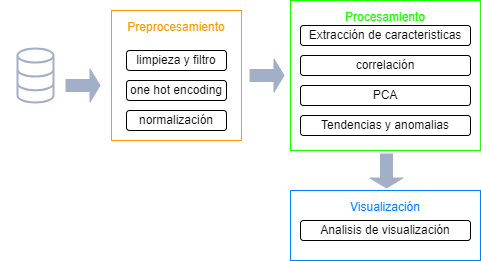
\includegraphics[width=\linewidth]{imagenes/pipeline.png} % Asegúrate de que "pipeline.png" exista en la carpeta "imagenes"
    \caption{Descripción general de pipeline de la propuesta para diagnosticar cancer pulmonar}
    \label{fig:pipeline}
\end{figure}


\begin{figure}[htb]
    \centering
    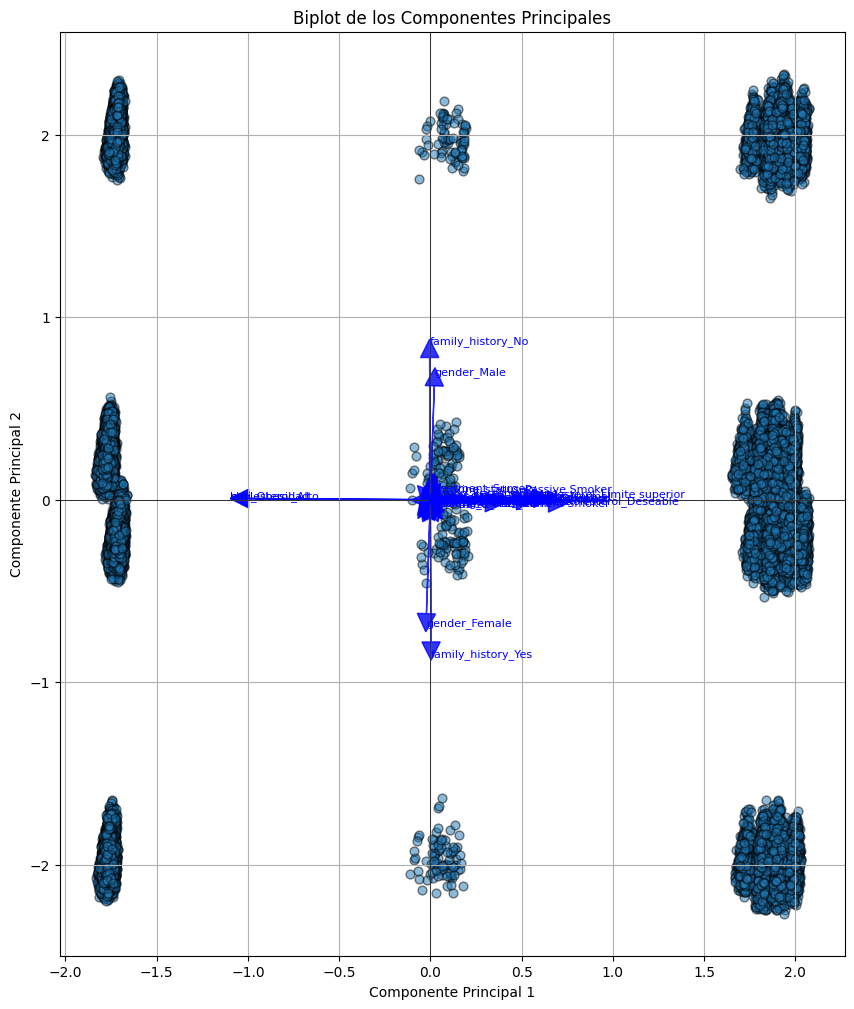
\includegraphics[width=\linewidth]{imagenes/pca_biplot.png}
    \caption{Resultado de la aplicación de PCA para reducir las variables a dos. Los vectores muestran el peso de cada variable por componente.}
    \label{fig:pca}
\end{figure}

\begin{figure}[htb]
    \centering
    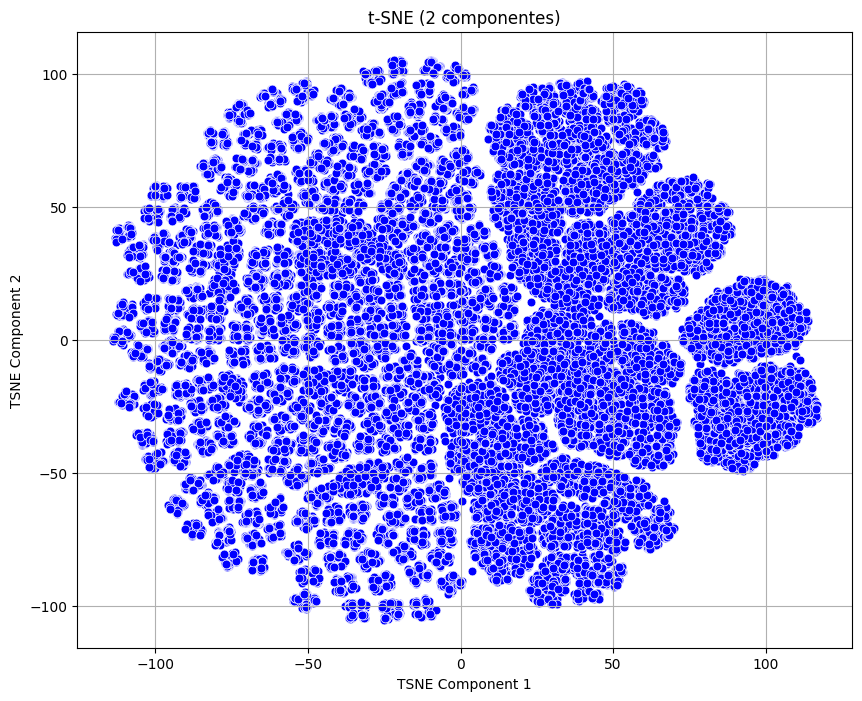
\includegraphics[width=\linewidth]{imagenes/tsne.png}
    \caption{Resultado de la aplicación de t-SNE. Se pueden apreciar agrupaciones de características.}
    \label{fig:tsne}
\end{figure}

\begin{figure}[htb]
    \centering
    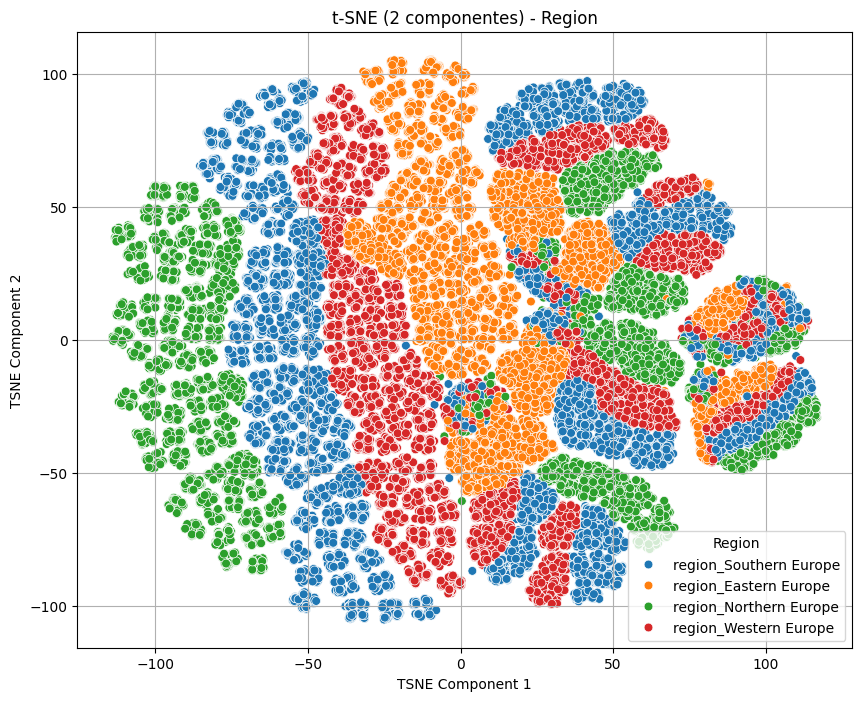
\includegraphics[width=\linewidth]{imagenes/region.png}
    \caption{Clusters según la región de Europa}
    \label{fig:tsne_region}
\end{figure}

\begin{figure}[htb]
    \centering
    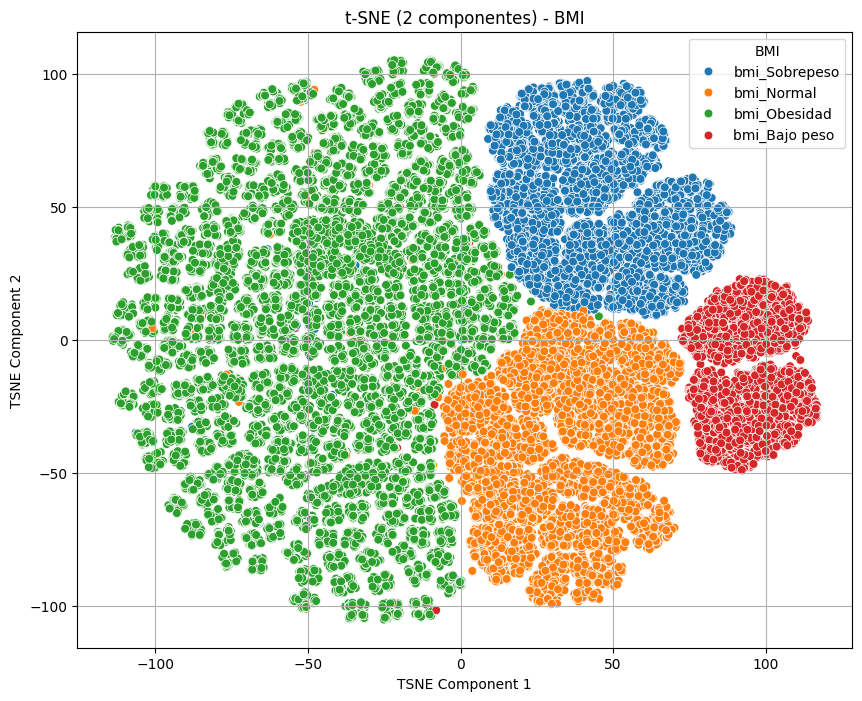
\includegraphics[width=\linewidth]{imagenes/bmi.png}
    \caption{Clusters de acuerdo al índice de masa corporal (BMI)}
    \label{fig:tsne_bmi}
\end{figure}

\begin{figure}[htb]
    \centering
    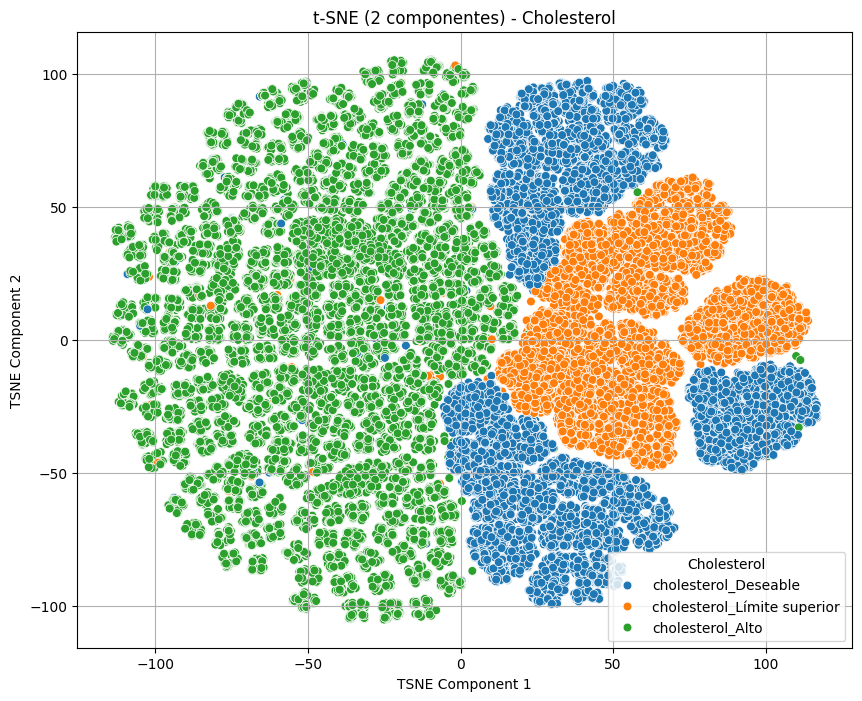
\includegraphics[width=\linewidth]{imagenes/cholesterol.png}
    \caption{Clusters de acuerdo al nivel de colesterol}
    \label{fig:tsne_cholesterol}
\end{figure}

\begin{figure}[htb]
    \centering
    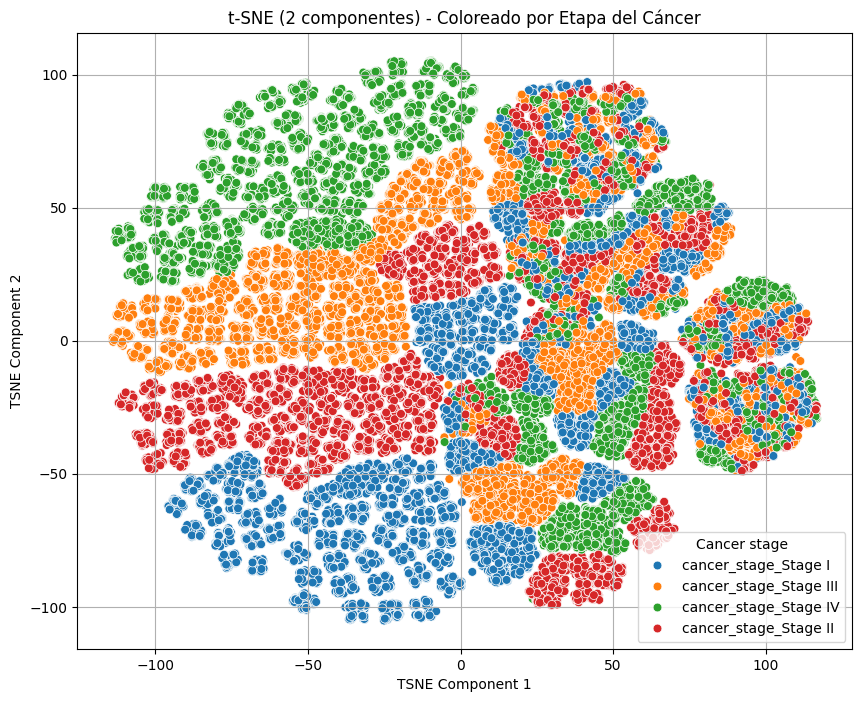
\includegraphics[width=\linewidth]{imagenes/cancer_stage.png}
    \caption{Clusters de acuerdo a la etapa diagnosticada de cáncer}
    \label{fig:tsne_cancer_stage}
\end{figure}

\begin{figure}[htb]
    \centering
    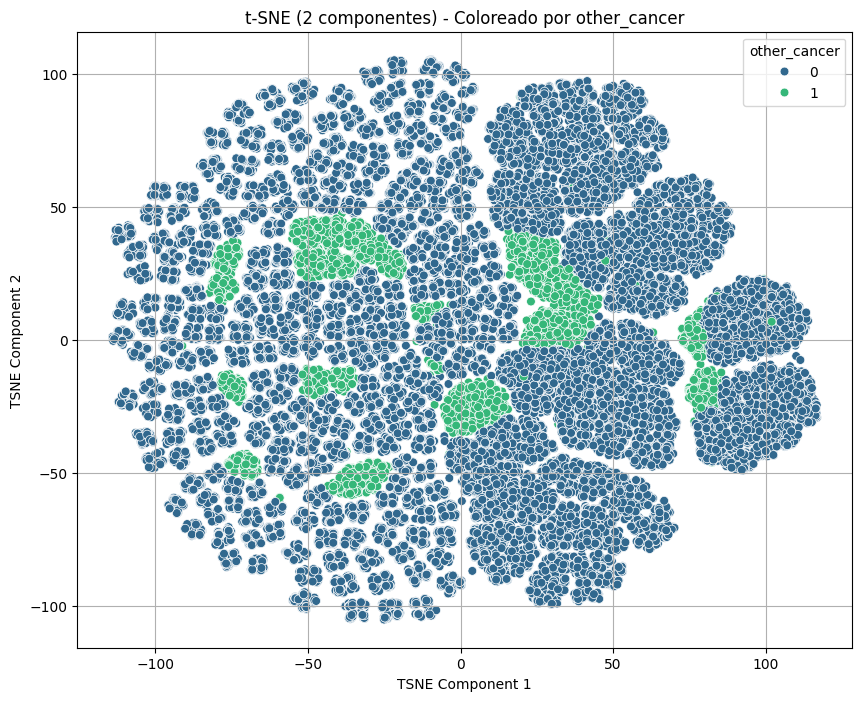
\includegraphics[width=\linewidth]{imagenes/other_cancer.png}
    \caption{Clusters de acuerdo a la presencia o no de otros tipos de cáncer}
    \label{fig:tsne_other_cancer}
\end{figure}


\section{Diseño Visual}
\section{Resultados}
\section{Discusión}
Según la imagen, podemos concluir que una persona con obesidad debería someterse a un chequeo preventivo de cáncer, ya que presenta una mayor probabilidad de desarrollar esta enfermedad.

\section{Conclusion}
The conclusion goes here.



\appendices
\section{Colab TrabajoCancerPulmon v2.ipynb}
Detalle de la aplicación
\begin{itemize}
  \item Lenguaje de Programación: Python
  \item Servidor: Google
  \item Librerias Principales; sklearn, matplotlib, pandas,seaborn, numpy
\end{itemize}
\href{https://colab.research.google.com/drive/1-HcDMOWJxGsakeZxqYCUc18EXPyz__4q?usp=sharing}{Codigo Colab} 
 


% use section* for acknowledgment
\ifCLASSOPTIONcompsoc
  % The Computer Society usually uses the plural form
  \section*{Acknowledgments}
\else
  % regular IEEE prefers the singular form
  \section*{Acknowledgment}
\fi


The authors would like to thank...

\ifCLASSOPTIONcaptionsoff
  \newpage
\fi

\begin{thebibliography}{1}

\bibitem{IEEEhowto:kopka}
H.~Kopka and P.~W. Daly, \emph{A Guide to {\LaTeX}}, 3rd~ed.\hskip 1em plus
  0.5em minus 0.4em\relax Harlow, England: Addison-Wesley, 1999.

\bibitem{ferraz2017}
R.~O.~Ferraz and D.~C.~Moreira-Filho, ``Análise de sobrevivência de mulheres com câncer de mama: modelos de riscos competitivos,'' \emph{Ciência \& Saúde Coletiva}, vol.~22, no.~11, pp.~3743--3754, Nov. 2017. [Online]. Available: https://doi.org/10.1590/1413-812320172211.05092016.

\bibitem{arxiv14031949}
Author(s) Name, "An Analysis of Machine Learning Models for Efficient Data Processing," \textit{International Journal of Computer Applications}, vol. 77, no. 3, pp. 33--38, 2013. [Online]. Available: \href{https://doi.org/10.48550/arXiv.1403.1949}{DOI: 10.48550/arXiv.1403.1949}.

\bibitem{jolliffe2016pca}
I.~T. Jolliffe and J.~Cadima, ``Principal component analysis: a review and recent developments,'' \emph{Philosophical Transactions of the Royal Society A: Mathematical, Physical and Engineering Sciences}, vol. 374, no. 2065, p. 20150202, 2016.

\bibitem{maaten2008tsne}
L.~van~der Maaten and G.~Hinton, ``Visualizing data using t-{SNE},'' \emph{Journal of Machine Learning Research}, vol.~9, pp. 2579--2605, 2008.

\bibitem{olsson1979maximum}
U.~Olsson, ``Maximum likelihood estimation of the polychoric correlation coefficient,'' \emph{Psychometrika}, vol.~44, no.~4, pp. 443--460, 1979.


\bibitem{aha_colesterol}
American Heart Association (AHA), ``Guideline on the Treatment of Blood Cholesterol to Reduce Atherosclerotic Cardiovascular Risk in Adults,'' \emph{American College of Cardiology}, 2018. [Online]. Available: https://www.heart.org/en/professional/education/guidelines-for-treatment-of-blood-cholesterol

\bibitem{cdc_bmi}
Centers for Disease Control and Prevention (CDC), ``Defining Adult Overweight and Obesity,'' \emph{CDC}, 2020. [Online]. Available: https://www.cdc.gov/obesity/adult/defining.html

\bibitem{nih_bmi_colesterol}
National Institutes of Health (NIH), ``Clinical Guidelines on the Identification, Evaluation, and Treatment of Overweight and Obesity in Adults,'' \emph{NIH}, 1998. [Online]. Available: https://www.nhlbi.nih.gov/files/docs/guidelines/obesity.pdf

\end{thebibliography}
 

\end{document}


